\documentclass[UTF8,a4paper,11pt]{ctexart}
\usepackage[left=2.50cm, right=2.50cm, top=2.50cm, bottom=2.50cm]{geometry} %页边距
\CTEXsetup[format={\Large\bfseries}]{section} 
 

% compile using Xelatex
%%%%%%%%%%%%%%%%%%%%%%%   字体备选栏
% -- 中文字体 --
%\setmainfont{Microsoft YaHei}  % 微软雅黑
%\setmainfont{YouYuan}  % 幼圆    
%\setmainfont{NSimSun}  % 新宋体
%\setmainfont{KaiTi}    % 楷体
%\setmainfont{SimSun}   % 宋体
%\setmainfont{SimHei}   % 黑体
% -- 英文字体 --
%\usepackage{times}
%\usepackage{mathpazo}
%\usepackage{fourier}
%\usepackage{charter}
\usepackage{helvet}
 
\usepackage{amsmath, amsfonts, amssymb} % math equations, symbols
\usepackage[english]{babel}
\usepackage{color}      % 控制文本颜色
\usepackage{graphicx}   % 加载图像包
\usepackage{url}        % 网址超链接
\usepackage{bm}         % equations的粗体形式
\usepackage{tikz}       % tikz 图像包
\usepackage{multirow}	% 列表设置一格多行多列
\usepackage{ulem}
\usepackage{booktabs}
\usepackage{epstopdf}
\usepackage{epsfig}
\usepackage{algorithm}  %编写算法

\usepackage{hyperref} %此处设置文本内超链接

%\usepackage{CJK,pgf,pgfarrows,pgfnodes,pgfautomata,pgfheaps}
\usepackage{amsmath,amssymb}
\usepackage{geometry}%页面设置
\usepackage{graphicx}%图片设置
\usepackage{float} %指定图片位置
%\usepackage{subfig}%多个子图
\usepackage{subfigure}%并排子图 共享标题 有子标题
\usepackage{caption}%注释设置

\usepackage{algorithm}
\usepackage{algorithmicx}
\usepackage{algpseudocode}  

% 这个和algorithmic不兼容,用了就要报错,好多莫名其妙的错误!!!!!
\floatname{algorithm}{算法}  
\renewcommand{\algorithmicrequire}{\textbf{输入:}}  
\renewcommand{\algorithmicensure}{\textbf{输出:}}  
\renewcommand{\algorithmicrequire}{ \textbf{Input:}}     %Use Input in the format of Algorithm
\renewcommand{\algorithmicensure}{ \textbf{Output:}}    %UseOutput in the format of Algorithm

\newtheorem{pf}{Pf}
\newtheorem{sol}{Sol}[section]
\newtheorem{thm}{Thm}
% 算法示例备选项
%\renewcommand{\algorithmicrequire}{ \textbf{Input:}}     % use Input in the format of Algorithm  
%\renewcommand{\algorithmicensure}{ \textbf{Initialize:}} % use Initialize in the format of Algorithm  
%\renewcommand{\algorithmicreturn}{ \textbf{Output:}}     % use Output in the format of Algorithm  

\DeclareMathOperator{\dif}{d\!}  %定义微分的缩写
\DeclareMathOperator{\pa}{\partial}  %定义偏微分的缩写

%\usepackage{fancyhdr}  %这里对 页眉、页脚 进行设置
%\pagestyle{fancy}
%\rhead{\thepage}
%\chead{}
%%\lhead{\includegraphics[width=1.6cm]{wallpaper.jpg}}
%\lfoot{}
%\cfoot{Page \thepage{} of \pageref{LastPage}}
%\rfoot{}
%
%\newcommand{\makeheadrule}{%        %去除页眉的横线 以免遮挡后面文字 
%	\makebox[0pt][l]{\rule[0\baselineskip]{\headwidth}{0pt}}%
%	\rule[0\baselineskip]{\headwidth}{0pt}}
%\renewcommand{\headrule}{%
%	{\if@fancyplain\let\headrulewidth\plainheadrulewidth\fi
%		\makeheadrule}}

%\usepackage[printwatermark]{xwatermark}   %%这以下设置“数学外卖”官方水印
%\usepackage{lipsum}
%
%\newsavebox\mybox
%
%\savebox\mybox{\tikz[color=gray,opacity=0.3]
%\newwatermark*[
%allpages,
%angle=48,
%scale=6,
%xpos=-20,
%ypos=15
%]{\usebox\mybox} 
 


\title{\textbf{Homework 2}}
\author{ 张思源  \qquad  \textit{21110850018} }   %这里填上您的大名


\begin{document}
\maketitle
\section{Ex1}
\textbf{某地成年人肥胖者($A_{1}$)占10\%,中等者($A_{2}$)占82\%,瘦小者($A_{3}$)占8\%,又有肥胖者,中等者,瘦小者高血压病的概率分别为20\%,10\%,5\%.\\
(1).求该地成年人患高血压的概率.\\
(2).若知某人患高血压,则他最可能属于哪种体型.}
\begin{sol}
	记患高血压和不患高血压分别为$B_{1},B_{2}$.\\
	$(1)$由题意,$P(B_{1}|A_{1})=0.2,P(B_{1}|A_{2})=0.1,P(B_{1}|A_{3})=0.05$.故由全概率公式:
	$$
	P(B_{1})=\sum_{i=1}^{3}P(B_{1}|A_{i})P(A_{i}).
	$$
	代入数据计算得$P(B_{1})=0.106=10.6\%$.\\
	即该地成年人患高血压的概率为$10.6\%$.\\
	$(2)$由题意及贝叶斯公式,该人肥胖的概率为:
	$$
	P(A_{1}|B_{1})=\frac{P(B_{1}|A_{1})P(A_{1})}{P({B_{1})}}=
	\frac{0.2\times0.1}{0.106}=0.1887,
	$$
	该人中等的概率为:
		$$
	P(A_{2}|B_{1})=\frac{P(B_{1}|A_{2})P(A_{2})}{P{(B_{1})}}=
	\frac{0.1\times0.82}{0.106}=0.7736,
	$$
	该人瘦小的概率为:
		$$
	P(A_{3}|B_{1})=\frac{P(B_{1}|A_{3})P(A_{3})}{P({B_{1}})}=
	\frac{0.05\times0.08}{0.106}=0.0377,
	$$
	所以该人最可能是中等体型.
\end{sol}
\section{Ex2}
\textbf{如教材3.54式和3.56式,分别写出如下有向图和无向图对应的概率分布.}
\begin{figure}[H]
	\centering
	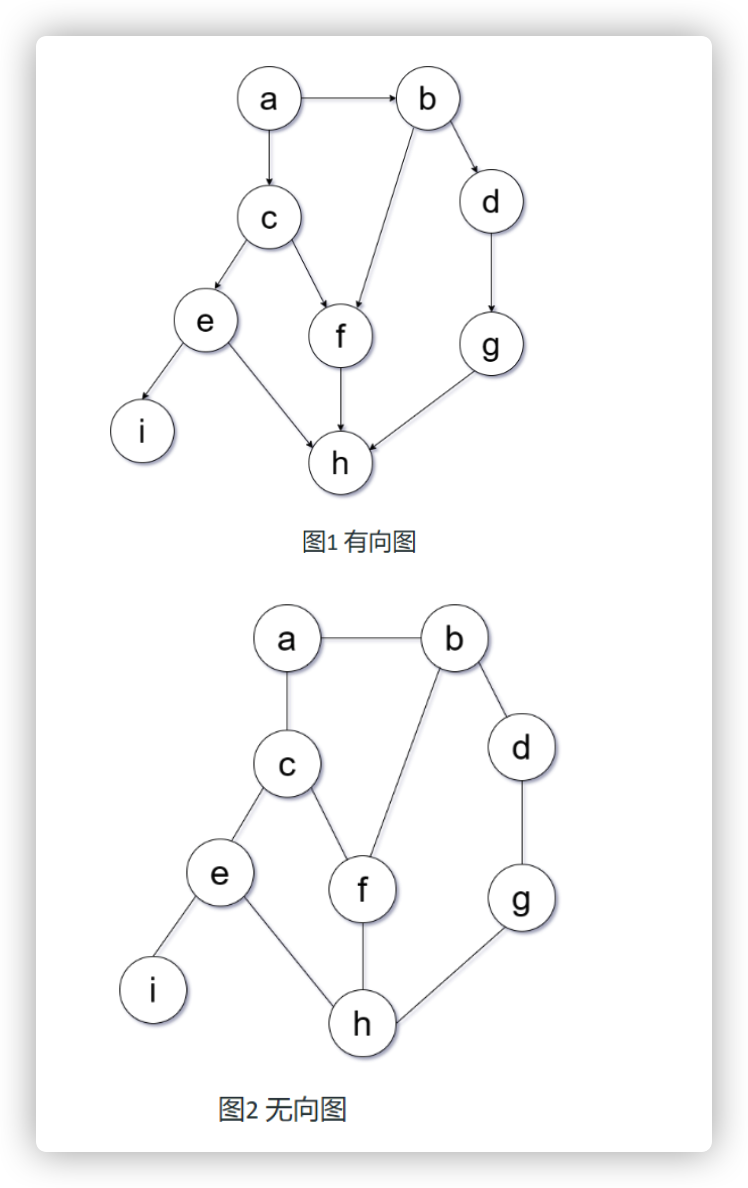
\includegraphics[width=0.7\textwidth,height=0.9\textwidth]{Ex2.png}
	\caption{Ex2}
\end{figure}
\begin{sol}
	对于有向图,$$p(a,b,c,d,e,f,g,h,i)=p(a)p(b|a)p(c|a)p(d|b)p(e|c)p(f|b,c)p(g|d)p(h|e,f,g)p(i|e).$$
	对于无向图,可以看出对于本模型,没有出现除了二阶子图之外的团,故其联合概率分布可写作\begin{equation*}
		\begin{split}
p(a,b,c,d,e,f,g,h,i)=&\frac{1}{Z}\phi^{(1)}(a,b)\phi^{(2)}(a,c)\phi^{(3)}(b,f)\phi^{(4)}(b,d)\phi^{(5)}(c,e)\\
	&\phi^{(6)}(e,h)\phi^{(7)}(g,h)\phi^{(8)}(d,g)
	\phi^{(9)}(e,i)\phi^{(10)}(c,f)\phi^{(11)}(f,h).
	\end{split}
	\end{equation*}
\end{sol}
\section{Ex3}
\textbf{取值为0,1,2,3,4,5的概率分别为1/2,1/4,1/8,1/16,1/32,1/32.求其香农熵.}
\begin{sol}
	由香农信息熵的定义:
	$$
	H(x)=-\sum_{i=0}^{5}P(x=i)\log_{2}(P(x=i))=\frac{31}{16}.
	$$
\end{sol}
\section{Ex4}
\textbf{叙述KL散度和交叉熵定义,并给出自己的理解.}
\begin{sol}
	KL-散度:设$p,q$是两个随机分布,则对于离散情况,$D_{KL}(p||q)=\sum_{k=1}^{K}p_{k}\log_{2}\frac{p_{k}}{q_{k}}$,对于连续情况,$D_{KL}(p||q)=\int_{\mathcal{X}}p(x)\log_{2}\frac{p(x)}{q(x)}dx$. KL-散度度量了使用基于$q$的分布来编码服从$p$的分布的样本所需的\textbf{额外的}平均比特数,之所以是额外是因为$p$与$q$的不匹配.\\
	交叉熵:设$p,q$是两个随机分布,则对于离散情况,$H(p||q)=-\sum_{k=1}^{K}p_{k}\log_{2}q_{k}$,对于连续情况,$H(p||q)=-\int_{\mathcal{X}}p(x)\log_{2}(q(x))dx$.交叉熵度量了使用基于$q$的分布来编码服从p的分布的样本所需的平均比特数(\textbf{这里不是额外的!!!}),从公式来看可以写作$D_{KL}(p||q)=H(p||q)-H(p)$,这反映了上述\textbf{"额外"}二字.\\
\end{sol}
\section{Ex5}
\textbf{说明每种分类器的含义以及区别并利用sklearning自带的数据集,自行划分训练集和测试集(无需验证集),使用第一种分类器(naive\_bayes.GaussianNB),并且可视化结果,说明在不同数据类型下分类器效果的差别.}
\begin{sol}
	$(1)$对于不同的朴素贝叶斯分类器,其含义及区别分别为:
	\begin{itemize}
	\item naive\_bayes.GaussianNB:高斯朴素贝叶斯,特征变量是连续变量且符合高斯分布:$$p(x_{i}|y)=\frac{1}{\sqrt{2\pi\sigma_{y}^{2}}}\exp(-\frac{(x_{i}-\mu_{y})^{2}}{2\sigma_{y}^{2})})$$
	\item naive\_bayes.BernoulliNB:多元伯努利朴素贝叶斯,模型适用于多元伯努利分布,即每个特征都是二值变量,如果不是二值变量,该模型可以先对变量进行二值化,特征变量满足分布:$$p(x_{i}|y)=p(i|y)x_{i}+(1-p(i|y))(1-x_{i})$$
	\item naive\_bayes.MultinomialNB:多项朴素贝叶斯,特征变量是离散变量,符合多项分布:$$\hat{\theta}_{yi}=\frac{N_{yi}+\alpha}{N_{y}+\alpha n}$$
	\item
	naive\_bayes.ComplementNB:是MultinomialNB模型的一个变种,实现了补码朴素贝叶斯(CNB)算法.CNB是标准多项式朴素贝叶斯(MNB)算法的一种改进,比较适用于不平衡的数据集.CNB使用来自每个类的补数的统计数据来计算模型的权重:
	\begin{equation*}
		\begin{split}
			\hat{\theta}_{ci}&=\frac{\alpha_{i}+\sum_{j:y_{j}\ne c}d_{ij}}{\alpha+\sum_{j:y_{j}\ne c}\sum_{k}d_{kj}}\\
			w_{ci}&=\log\hat{\theta_{ci}}\\
			\hat{w}_{ci}&=\frac{w_{ci}}{\sum_{j}|w_{cj}|}
		\end{split}
	\end{equation*}
	\end{itemize}
$(2)$
\begin{figure}[H]
	\centering
	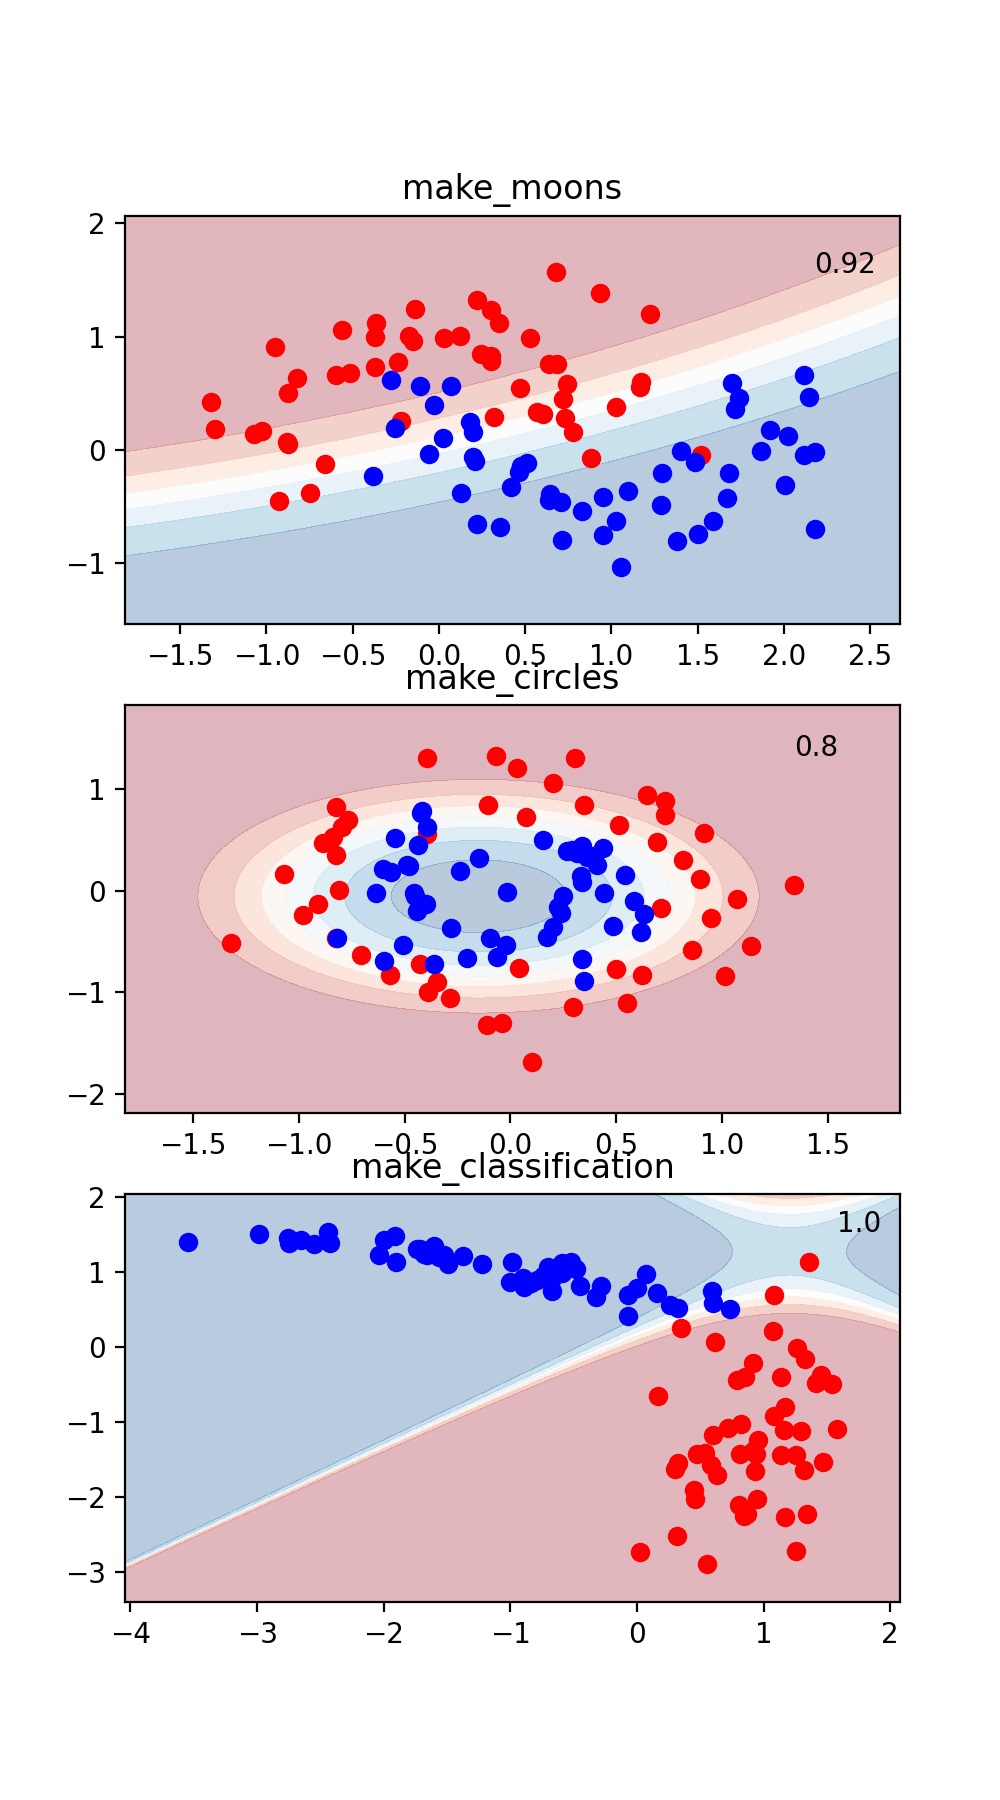
\includegraphics[width=0.7\textwidth,height=1.2\textwidth]{1.png}
	\caption{numerical experiment 1}
\end{figure}
\begin{figure}[H]
	\centering
	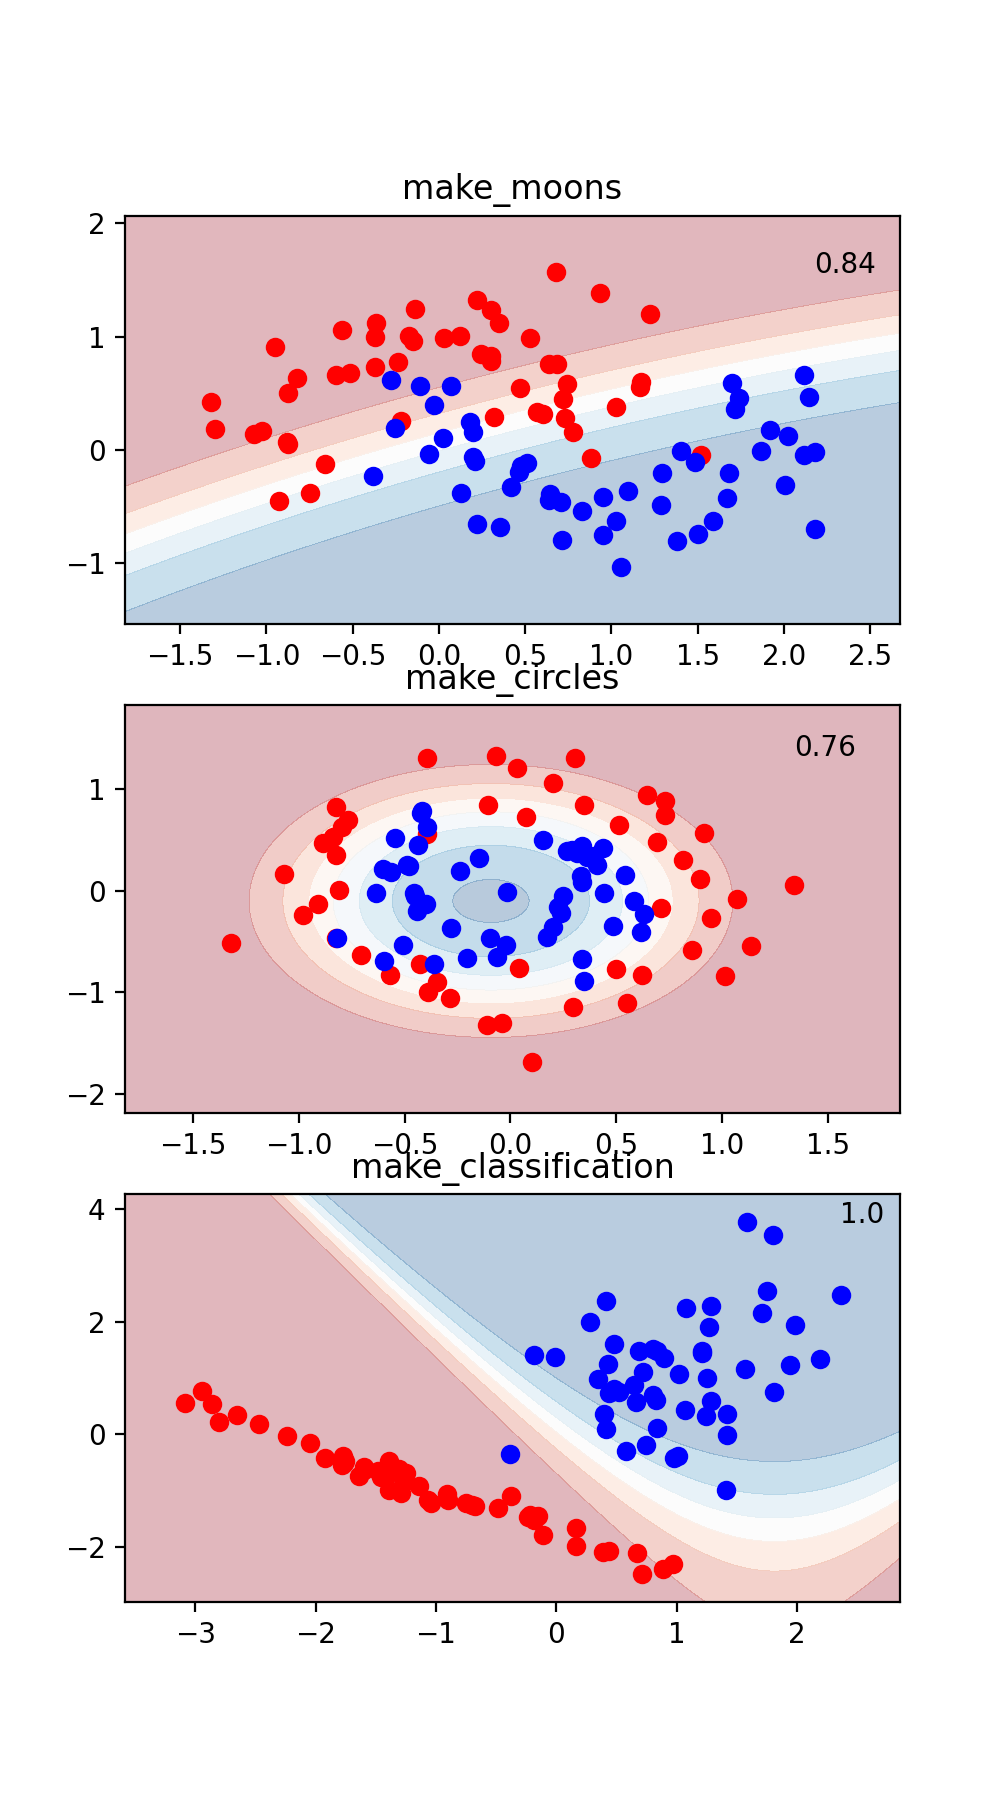
\includegraphics[width=0.7\textwidth,height=1.2\textwidth]{2.png}
	\caption{numerical experiment 2}
\end{figure}
\par 可以看出,在naive\_bayes.GaussianNB分类器下,对于近似线性可分的make\_moons数据集和线性可分的make\_classification数据集的分类效果较好,对非线性可分的make\_circles数据集的分类效果较差.月牙形数据集的分类边界大概为正弦函数$\frac{1}{4}$的曲线,这与其正弦形的形状可能有关;圆环形数据集的分类边界大概为圆环,且内部为蓝色,外部为红色,这与数据的分布基本一致;线性可分数据集的分类边界大概为线性函数的组合,这可能是与其数据的生成方式有关,同时由于该数据集的线性可分性,其具有最好的可分性质,换言之,分类器在测试集上的准确率最高.

\textbf{一方面,这可能是因为对于线性可分的数据集,其先验概率的计算(或者说估计)更为接近高斯分布;另一方面,这可能是因为对于make\_moons和make\_classification数据集其每一特征重要性接近,或者说权重相当.}
\end{sol}
\newpage
\begin{thebibliography}{3}  
	\bibitem{ref1} 李航. 统计学习方法[M]. 清华大学出版社, 2012.
	%\bibitem{ref2} Kingma D , Ba J . Adam: A Method for Stochastic Optimization[J]. Computer Science, %2014.
	\bibitem{ref2} Goodfellow, Ian, et al. Deep Learning[M]. MIT Press, 2016. 	
\end{thebibliography}
\end{document}
